\documentclass{article}
\usepackage[letterpaper, portrait, margin=1.0in]{geometry}
\usepackage{graphicx}
\graphicspath{ {./} }


\title{CMSC 471 - Project 3}
\date{2016-05-02}
\author{Jerson Guansing}

\begin{document}
  \pagenumbering{gobble}
  \maketitle
  \newpage
  \tableofcontents
  \newpage
  \pagenumbering{arabic}

  \section{Project Overview}
  
  Your program should take a single argument, the filepath to a jpg. It will then print out one of the following strings:\\
  \begin{enumerate}
  	\item Smile
  	\item Hat
  	\item Dollar
  	\item Hash
  	\item Heart
  \end{enumerate}
  You should include a readme explaining how to run and / or install your program. You should also include a report describing your approach, your accuracy, and anything else you think would be of interest. This will likely be between two or three pages, and should be written in latex.\\
  
  \section{Goal}
  
  The main goal of this project is to apply the lessons about supervised learning, and find the best approach to accurately perform image classification.
  
  
  \section{Training and Testing Sets}
  
  All the images provided are 100 x 100 jpeg files with the exception of Smile/01.jpg which was removed from the data set for consistency.\\
  
  The image count for each category are as follow:\\
  \begin{enumerate}
  	\item Smile: 84 images (It was 85, but removed one file that is not 100 x 100)
  	\item Hat: 72 images
  	\item Dollar: 87 images
  	\item Hash: 88 images
  	\item Heart: 81 images
  \end{enumerate}
  
  For the training set, the first 60 images for each category was used as the independent and identically distributed (iid) samples. However, a different approach was done for the testing sets. The test runs were conducted with two test sets: (1) 12 unused images for each category as the independent and identically distributed samples since there are only 72 hat images, and (2) all the unused images for each category which is an uneven distribution of sample.
  
  \begin{enumerate}
  	\item Training Set: 300 images (60 images per category)
  	\item Test Set 1: 60 images (12 images per category that were not used in the training set)
  	\item Test Set 2: 117 images (All images per category that were not used in the training set)
  \end{enumerate}
  
  \section{Featurization}
  
  All the image sets need to be converted to a matrix / np.array. The main approach used was to flatten the images by averaging the rgb values of each pixel, and essentially turning it to a  gray scale image. This makes the training set smaller and a little more efficient since it is working with 1 value per pixel for an image that is 100 x 100 (10,000 array length). The array of images are then stored as X (n sample, n features) while the label/category for each image is stored as Y, and then fitted to classifiers K-Neighbors and SVMs for the training set.\\
  
  Another approach that was tested is shrinking the 10,000 pixel images to 100 by averaging the vertical pixels of each image. There are less components to work with for the training sets making it faster, but loses some detail. Similarly, exponential trick (squaring, cubing, etc.) was tested to try to make the data points more linearly separable, but only resulted in accuracy loss.
  
  
  \section{Result}
   
    \subsection{Test Set Result}
   \begin{table}[h]
  	\centering
  	\caption{Test Set Result}
  	\label{tab:table1}
  	\begin{tabular}{|c|c|c|c|c|}
  	\hline
  	Method & Test1: Correct & Test1: Incorrect & Test2: Correct & Test2: Incorrect \\
  	\hline
  	SVM kernel=linear & 56 & 4 & 105 & 12 \\
  	\hline
  	SVM kernel=rbf & 33 & 27 & 59 & 58 \\
  	\hline
  	SVM kernel=poly, degree=3 & 56 & 4 & 107 & 10 \\
  	\hline
  	K-Neighbors & 60 & 0 & 113 & 4 \\
  	\hline
  \end{tabular}
  \end{table}
  
  \subsection{Which did better}
  The results listed on Table 1 uses a training set with samples featured with the full 10,000 pixels (100 x 100 image) where each pixel is the average rgb values. The best result came from using the K-Neighbors classifier with a 100\% accuracy using the independent and identically distributed (iid) testing set sample (Test 1), and the second test using the unevenly distributed sample (Test 2 set) still yielded 96.6\% accuracy. The accuracy for the polynomial and linear SVMs is 93.3\% which is respectable, but not as good as the K-Neighbors classifier using the iid sample set. However, the SVM using an rbf (radial basis) kernel did so poorly compared to the other methods with only a 55\% accuracy. Looking at the graph representation of the training set, there are a lot of overlapping data points which makes drawing boundaries between categories harder.\\
 
 \subsection{Other Trials}
 These other trials manipulating the training set's sample data resulted in lower or the same accuracy. There were no significant indicators to justify using these methods (more computation) for the same or less accuracy result.
 \begin{table}[h]
 	\centering
 	\caption{Other Trials}
 	\label{tab:table2}
 	\begin{tabular}{|c|c|c|c|c|}
 		\hline
 		Method & Test1: Correct & Test1: Incorrect & Test2: Correct & Test2: Incorrect \\
 		\hline
 		Exponential, n=2 & 60 & 0 & 113 & 4 \\
 		\hline
 		Vertical Average & 54 & 6 & 97 & 20 \\
 		\hline
 		Vertical Average and Exponential n=7 & 56 & 4 & 104 & 13 \\
 		\hline
 	\end{tabular}
 \end{table}
  \newpage
  
 \section{Graphs}
 
 \subsection{One Image per Category: 10,000 pixels per image}
 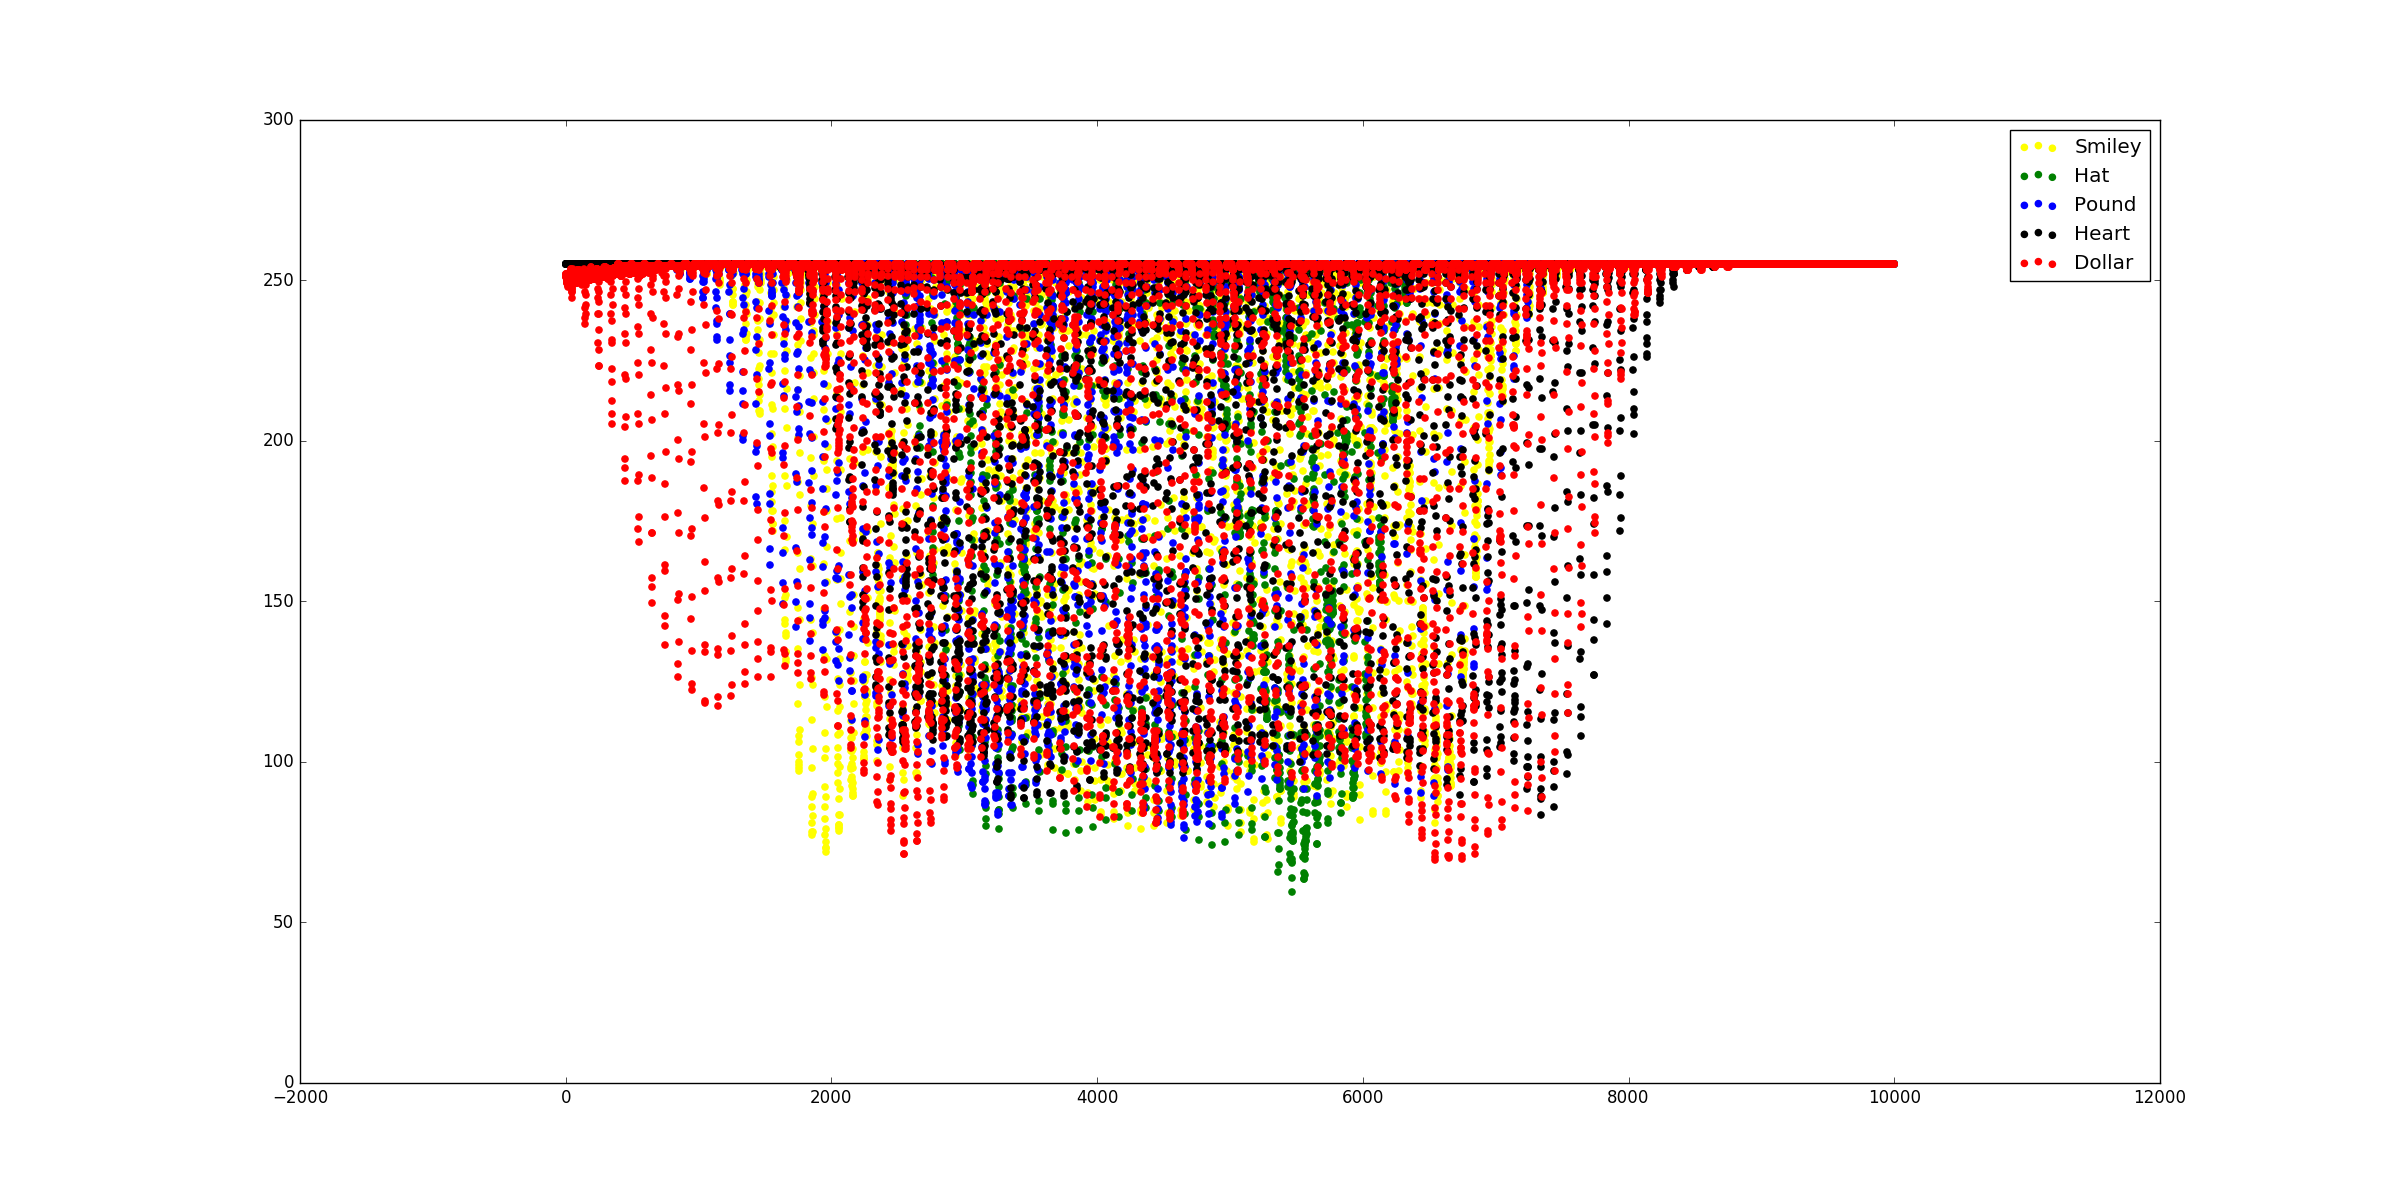
\includegraphics[width=1.1\textwidth]{figure_1.png}
 
 This is a graphical representation of the base training set using only 1 image per category. This highlights the data plots that overlap, and points out certain spots that are unique for each category.

 \subsection{All Images in the Training Set: 10,000 pixels per image}
 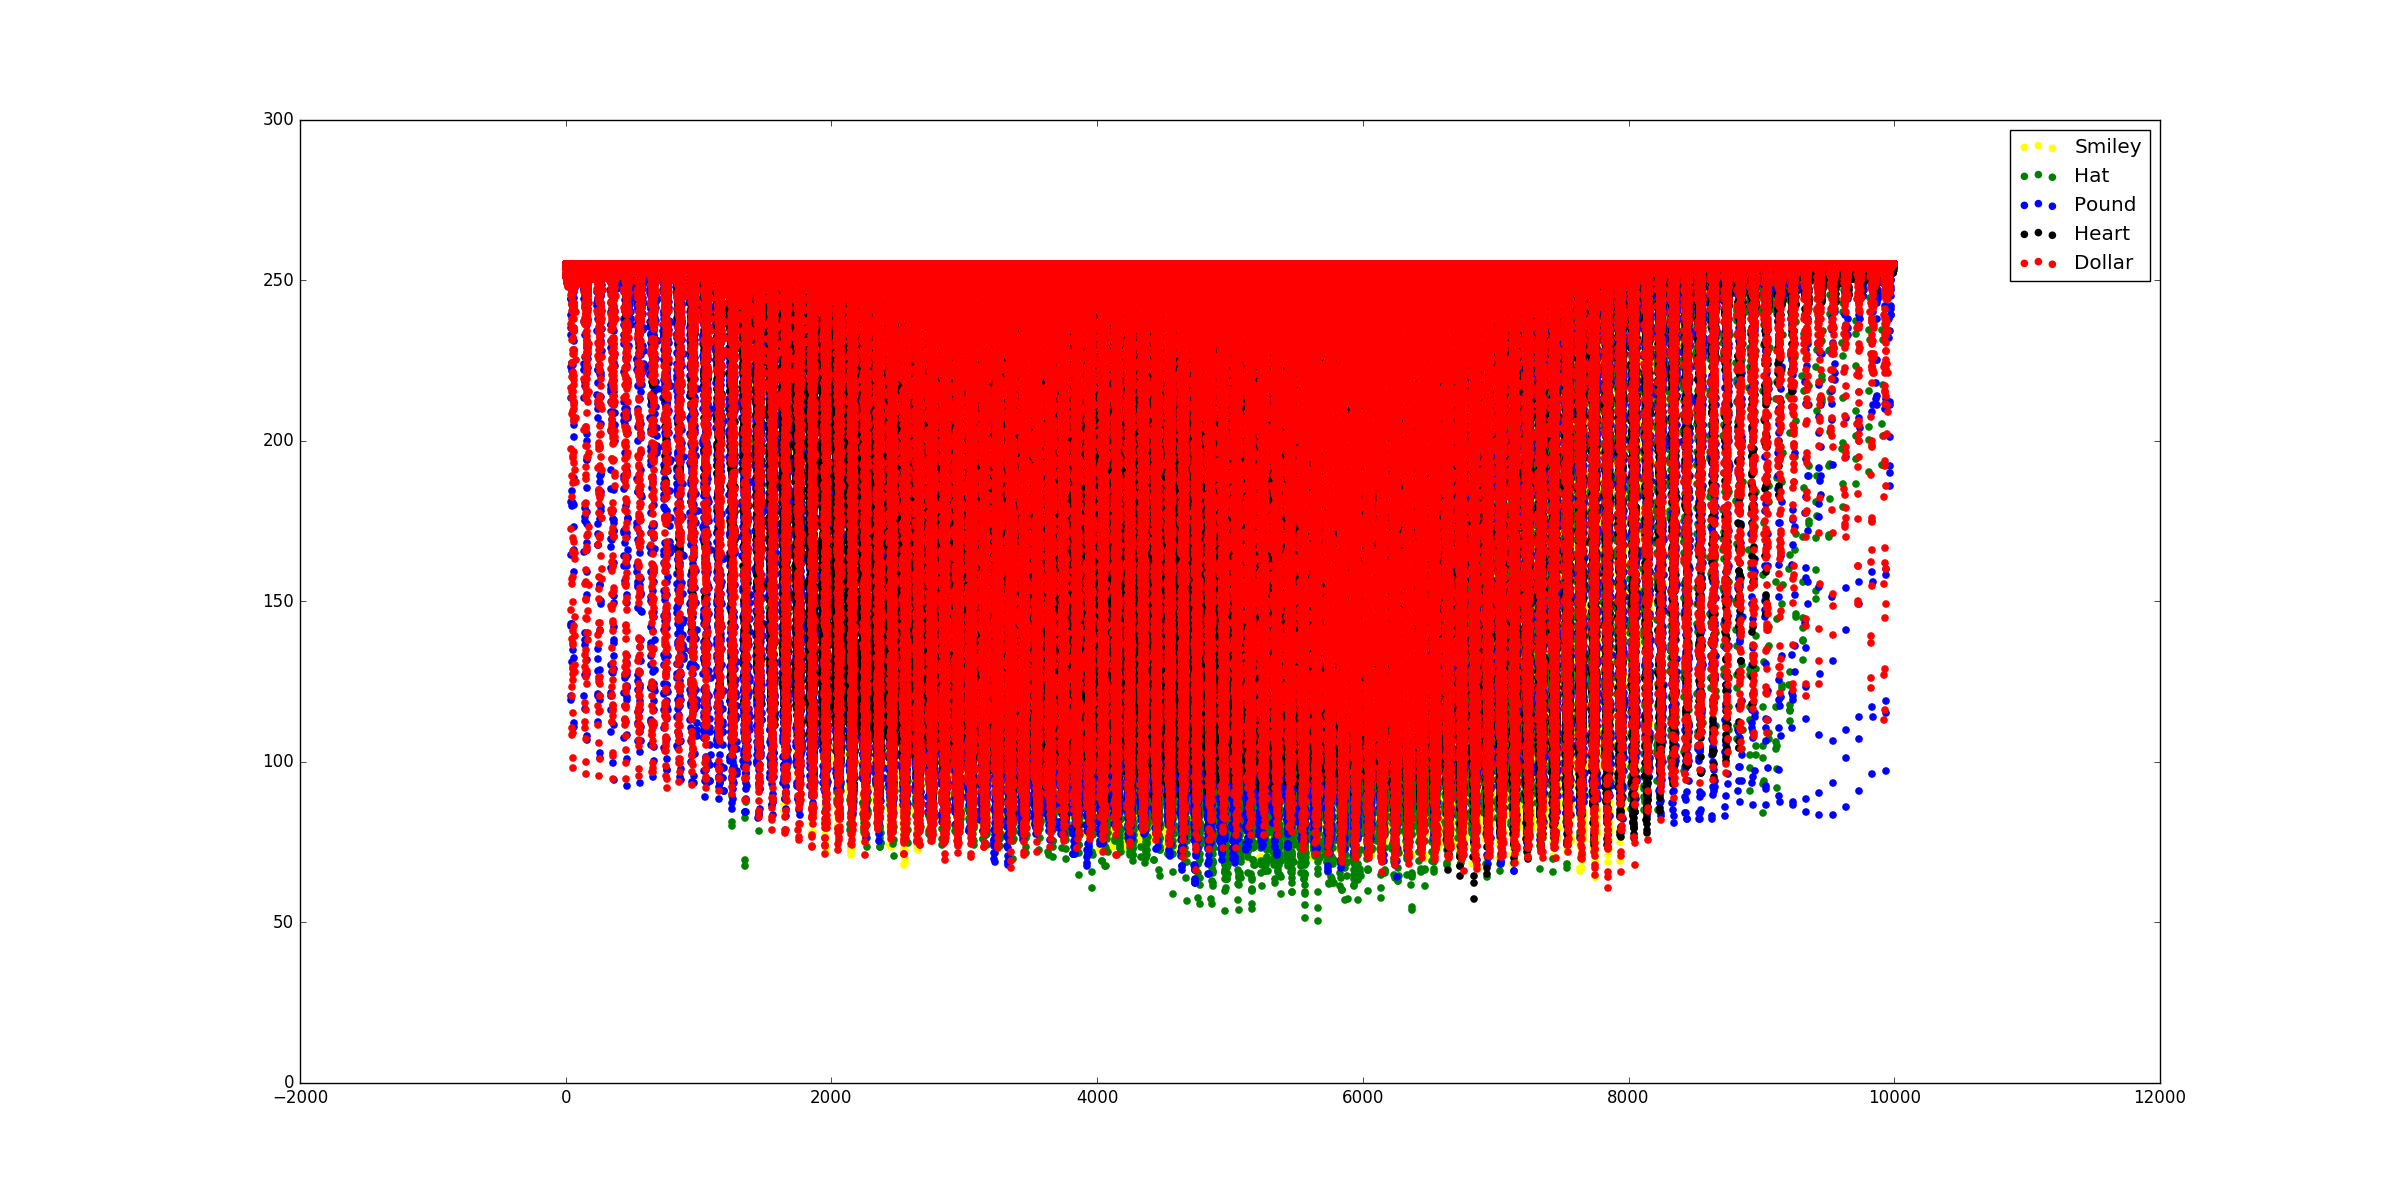
\includegraphics[width=1.1\textwidth]{figure_2.png}

  \subsection{Other Trial - Exponential n=2: 10,000 pixels per image}
  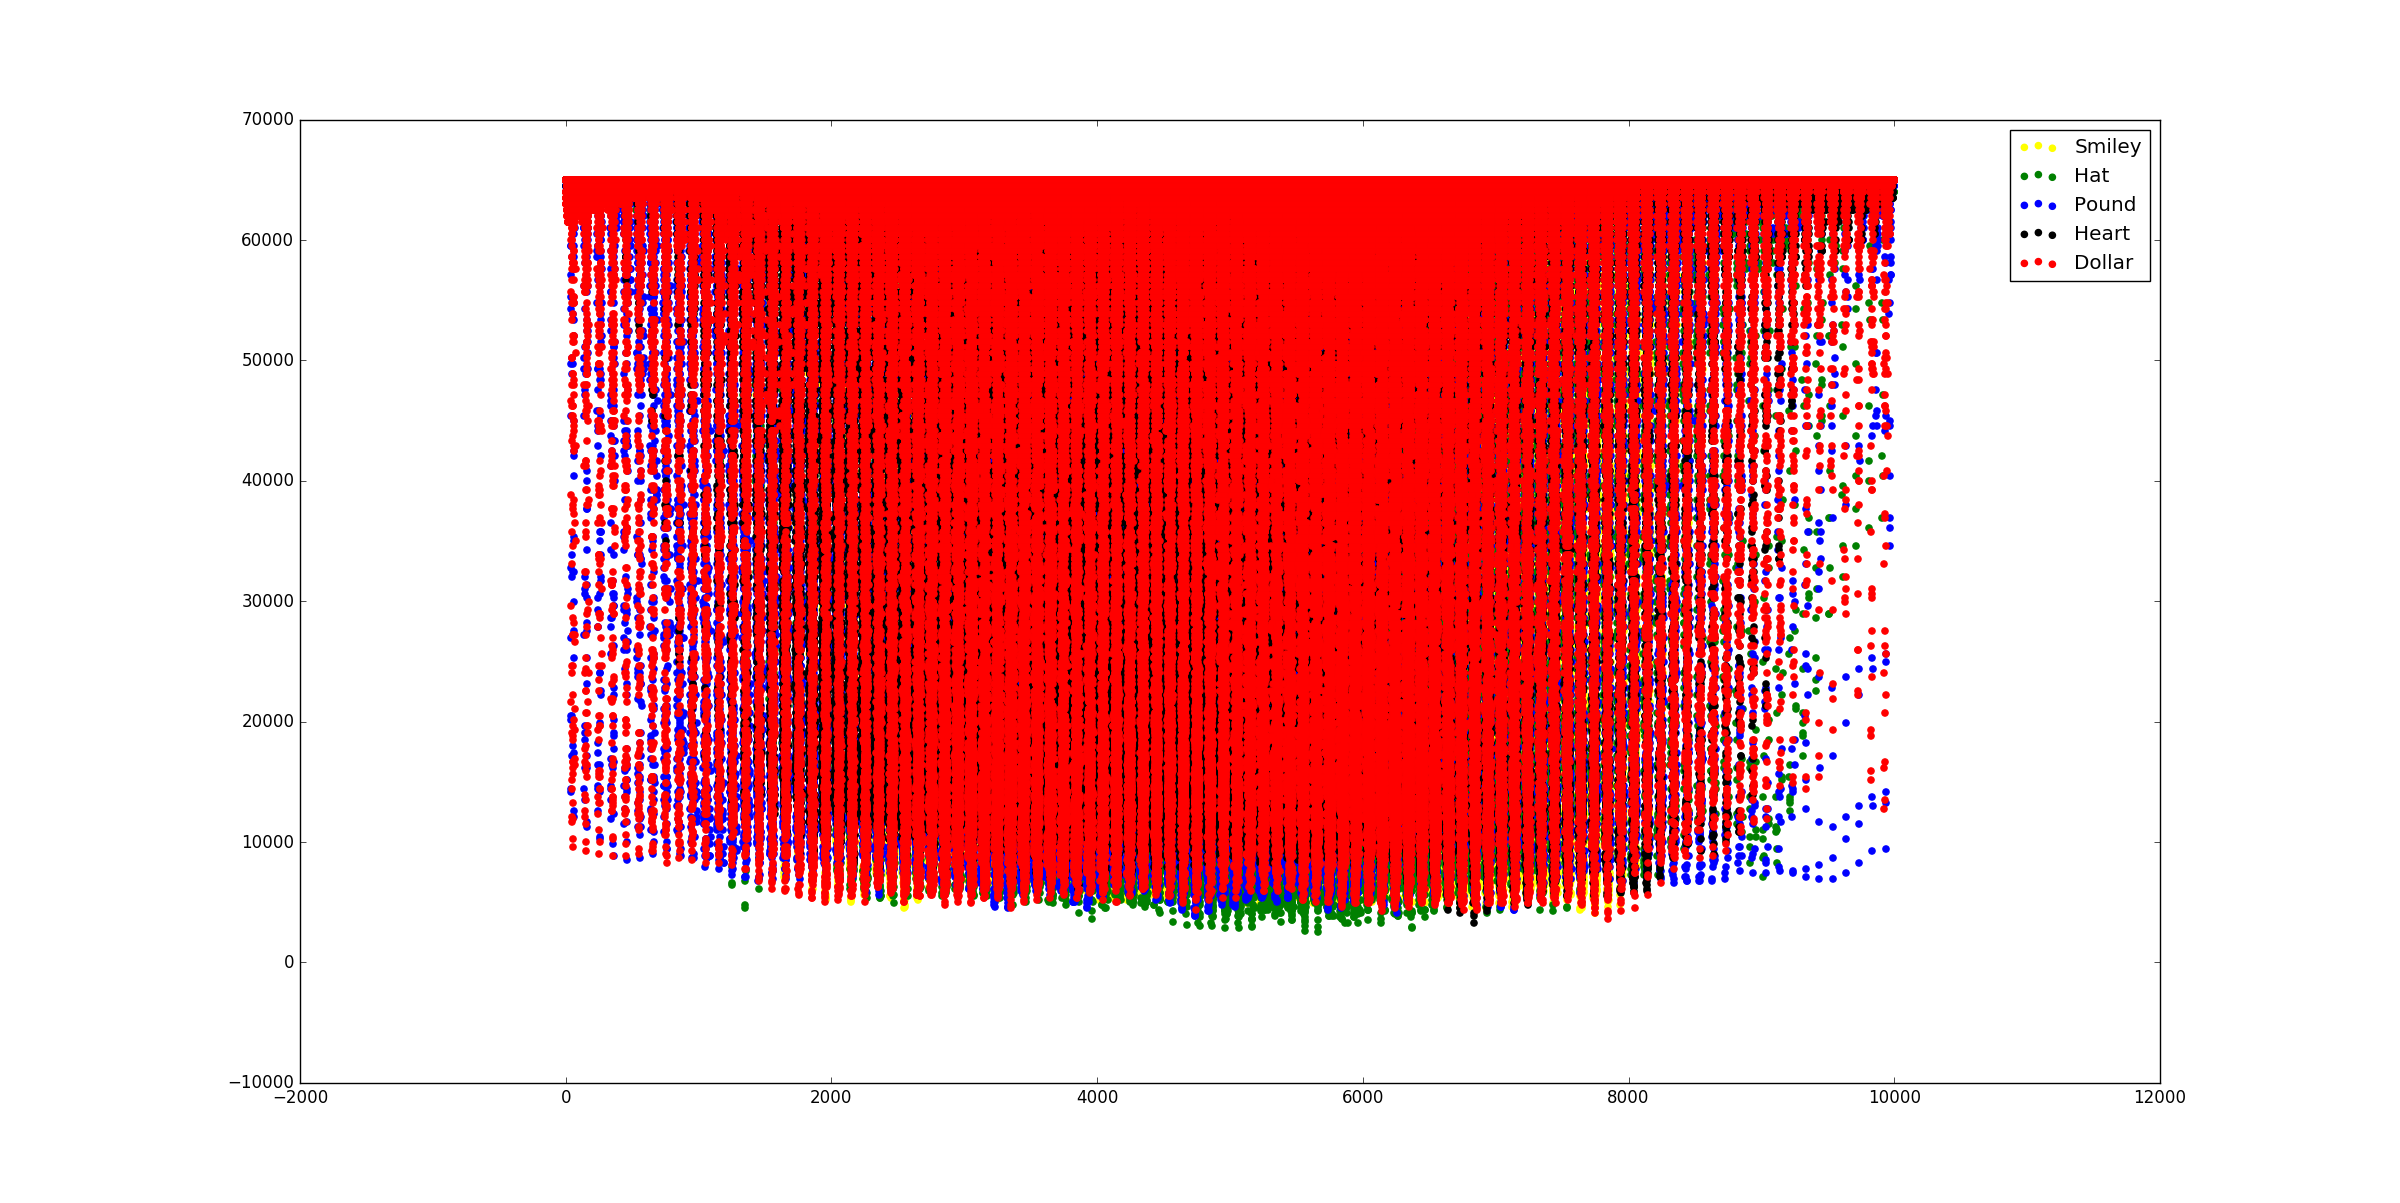
\includegraphics[width=1.1\textwidth]{figure_3.png}
  
  There was no  difference raising the data plots to the power n compared to the results of just running a K-Neighbors classifier with the base training set. This method will just take more computation readjusting the data values for the same result.
  
  \subsection{Other Trial - Vertical Average: 100 pixels per image}
  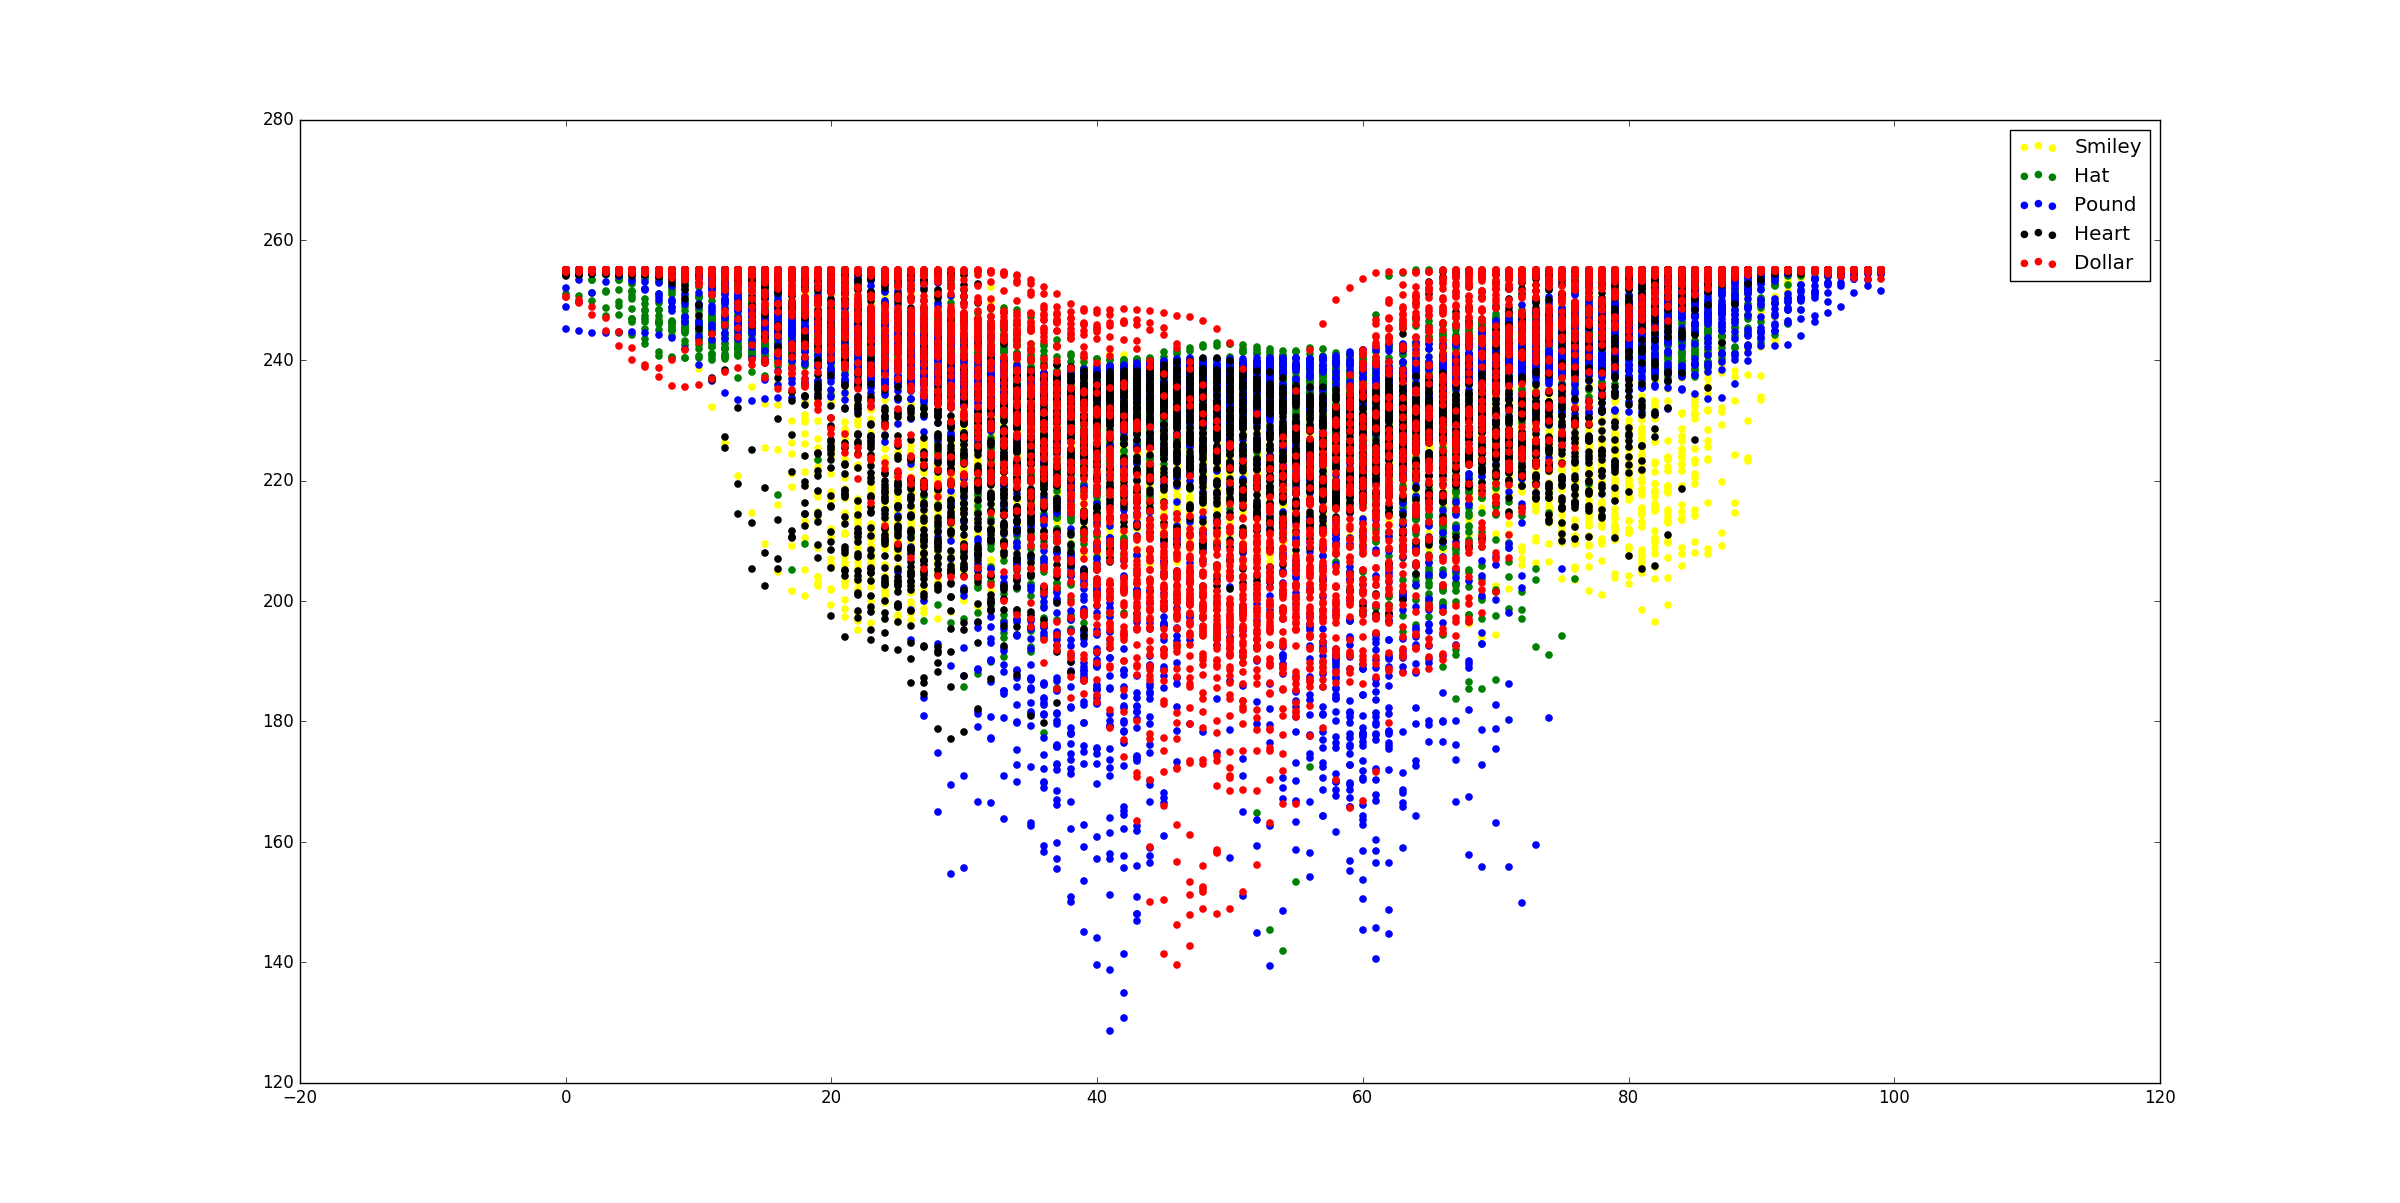
\includegraphics[width=1.1\textwidth]{figure_4.png}
  
  The 10,000 pixel image (100 x 100) was shrunk by getting the vertical average of the data, and essentially reducing the image to a 100 length array. Result-wise, it is below a K-Neighbor classifier method using the base training set.
  
  \subsection{Other Trial - Exponential n=7: 100 pixels per image}
  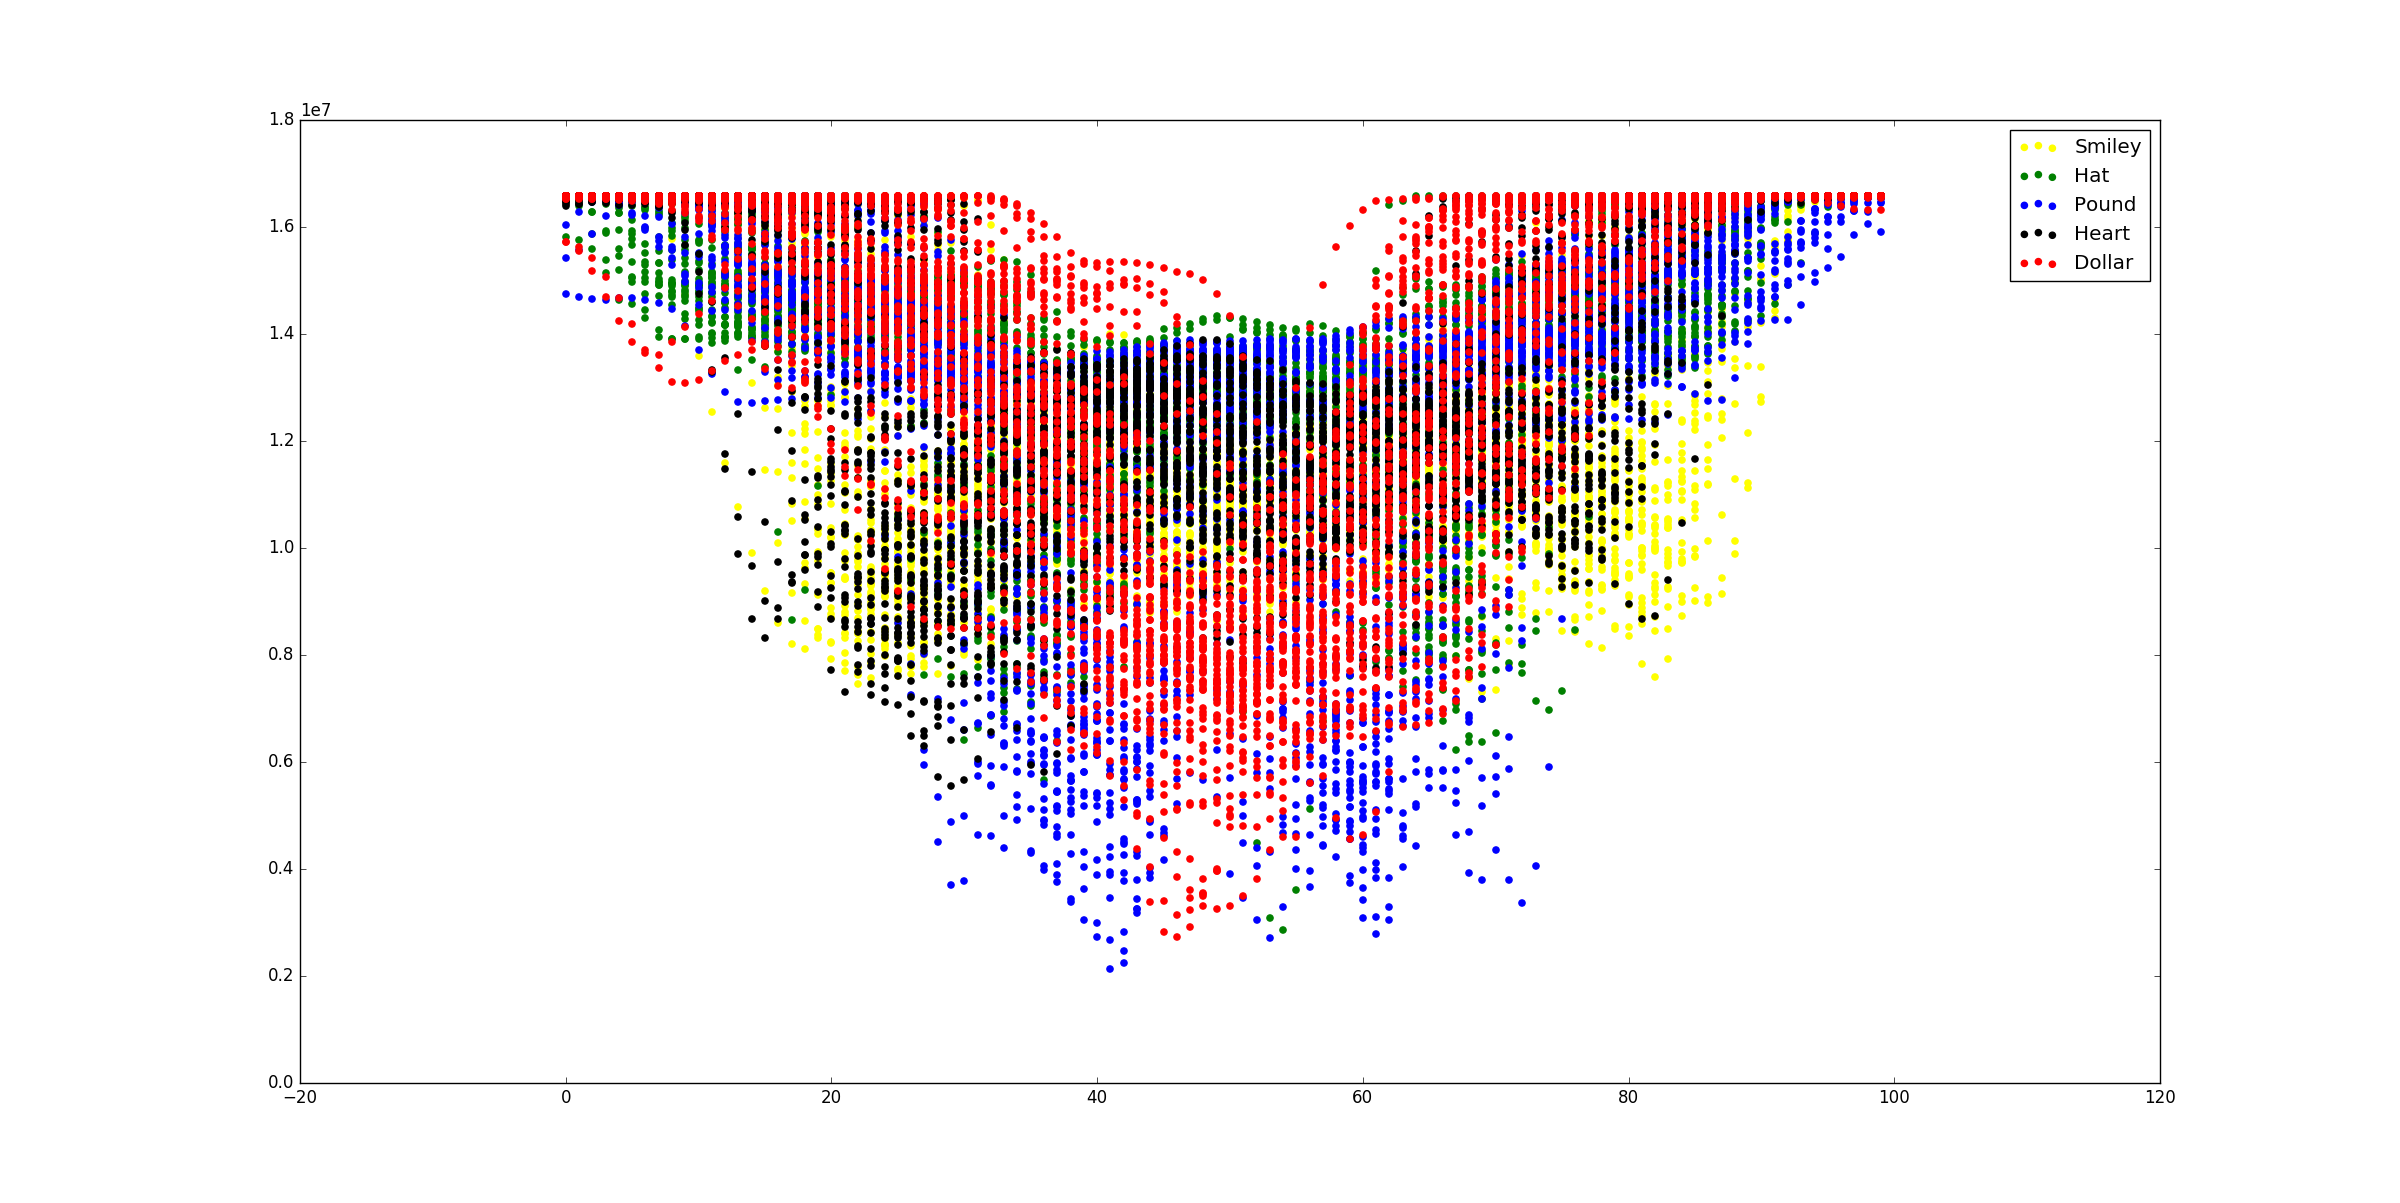
\includegraphics[width=1.1\textwidth]{figure_5.png}
   
   Combining both vertical average and exponential yielded an accuracy result that is still below the prescribed method using K-Neighbors classifier with the base set. The detail loss from the vertical averaged pixels affected the accuracy way too much, and even after raising it to an n power was not enough to compensate for the accuracy loss.
	  
\end{document}